\documentclass{article}
\usepackage[utf8]{inputenc}
\usepackage[spanish]{babel}
\usepackage{graphicx}
\usepackage{hyperref}
\usepackage{amsmath}
\usepackage{geometry}
\usepackage{booktabs}
\usepackage{adjustbox}
\usepackage{caption}
\usepackage{multirow}
\usepackage{pdflscape}
\usepackage{float}
\usepackage{array}
\geometry{a4paper, margin=1in}

\hypersetup{
    colorlinks=true,
    linkcolor=black,
    urlcolor=blue,
    citecolor=black
}

\title{MPI sobre clúster AWS: multiplicación de matrices con paso de mensajes\\[0.5em]
\large Caso de Estudio 3 --- Computación de Alto Rendimiento}
\author{Daniel Toro Soto , Juan Camilo Galvis}
\date{Mayo 2026}

\begin{document}

\maketitle

\begin{abstract}
El presente documento describe la implementación, despliegue y análisis de desempeño de una versión paralela con MPI (\emph{Message Passing Interface}) del algoritmo de multiplicación de matrices cuadradas en lenguaje C, ejecutada sobre un clúster real desplegado con AWS ParallelCluster. La infraestructura consta de un nodo \emph{HeadNode} de orquestación y tres nodos de cómputo \texttt{c7i-flex.large} (2 vCPUs y 8\,GB de RAM por nodo, para un total de 6 vCPUs distribuidas), administrados por Slurm y comunicados a través de un sistema de archivos compartido EFS montado por NFS. Se ejecutaron 11 tamaños de matriz (entre 504 y 4008) con 7 repeticiones por configuración para tres niveles de paralelismo (2, 4 y 6 procesos MPI), tomando como línea base un binario secuencial monolítico. Los resultados muestran que la implementación punto a punto escala de manera consistente al aumentar el número de procesos y que el clúster alcanza speedups cercanos a $8.7\times$ para matrices de $4008 \times 4008$ usando los 6 procesos disponibles.
\end{abstract}

\tableofcontents
\newpage

% ─────────────────────────────────────────────────────────────────────────────
\section{Introducción}

La computación de alto rendimiento (HPC) busca resolver problemas de gran escala distribuyendo el trabajo entre múltiples recursos de cómputo. En casos de estudio previos del curso, la multiplicación de matrices cuadradas se paralelizó sobre una sola máquina, aprovechando memoria compartida mediante hilos POSIX y procesos creados con \texttt{fork()}. En este caso de estudio se da un paso adicional: la paralelización se realiza sobre memoria \emph{distribuida}, donde los procesos no comparten espacio de direcciones y deben comunicarse explícitamente por la red mediante un estándar de paso de mensajes.

El estándar utilizado es MPI (\emph{Message Passing Interface}), específicamente la implementación OpenMPI provista por la distribución Amazon Linux 2 del clúster. El despliegue de la infraestructura se realiza con \texttt{aws-parallelcluster}, una herramienta oficial de AWS que abstrae la creación de un \emph{HeadNode}, los nodos de cómputo y el almacenamiento compartido EFS necesarios para ejecutar trabajos paralelos sobre Slurm. El enunciado del caso de estudio exige un mínimo de 3 nodos de cómputo y advierte explícitamente que la medición de tiempo no debe usar relojes de pared locales en cada nodo, sino el mecanismo propio de MPI (\texttt{MPI\_Wtime}).

El objetivo de este informe es: (i) documentar la infraestructura del clúster y el proceso de despliegue; (ii) describir el algoritmo MPI punto a punto implementado; (iii) reportar los tiempos de ejecución y speedups obtenidos para 11 dimensiones de matriz y 3 niveles de paralelismo; y (iv) analizar el comportamiento de escalabilidad observado al variar el número de procesos.

% ─────────────────────────────────────────────────────────────────────────────
\section{Marco Conceptual}

\subsection{High Performance Computing (HPC)}

Cuando hablamos de HPC ``hacemos referencia a un campo de la computación actual que da solución a problemas tecnológicos muy complejos y que involucran un gran volumen de cálculos o de coste computacional'' (López, 2017)\cite{lopez}. El producto matricial es un problema de referencia para evaluar HPC porque su complejidad cúbica crece muy rápido con la dimensión de la matriz, lo que justifica explorar estrategias de paralelización tanto en memoria compartida como en memoria distribuida.

\subsection{Multiplicación matricial}

Dadas dos matrices cuadradas $A$ y $B$ de dimensión $n$:

\[ A := (a_{ij})_{n \times n} \qquad B := (b_{ij})_{n \times n} \]

el producto $C = AB$ genera una matriz $C := (c_{ij})_{n \times n}$ donde

\[ c_{ij} = \sum_{k=1}^{n} a_{ik} \cdot b_{kj}. \]

El algoritmo ingenuo consiste en tres bucles anidados, con complejidad temporal $\mathcal{O}(n^3)$ y espacial $\mathcal{O}(n^2)$ (Cortéz, 2004)\cite{cortez}.

\subsection{Computación distribuida vs. memoria compartida}

En memoria compartida, los hilos o procesos viven dentro de una misma máquina y comparten un mismo espacio de direcciones (o bien lo simulan vía \texttt{mmap}). El costo de comunicación entre trabajadores es bajo: basta con escribir y leer la misma región de memoria. En memoria distribuida, cada proceso vive en una máquina distinta y la única forma de coordinarse es enviar mensajes a través de la red. Esto introduce un \emph{overhead} de comunicación que no existía en los casos anteriores, pero a cambio permite escalar el problema más allá del límite de una sola máquina (Ferestrepoca, 2019)\cite{ferestrepoca}.

\subsection{MPI: Message Passing Interface}

MPI es el estándar \emph{de facto} para programación paralela en memoria distribuida. Define una API en C/Fortran/Python que abstrae el paso de mensajes entre procesos independientes, y oculta los detalles del medio de transporte subyacente (TCP, UDP, InfiniBand, etc.). Sus elementos fundamentales son:

\begin{itemize}
    \item \textbf{Communicator}: grupo lógico de procesos que pueden intercambiar mensajes. El comunicador por defecto es \texttt{MPI\_COMM\_WORLD} y agrupa a todos los procesos lanzados por \texttt{mpirun}.
    \item \textbf{Rank}: identificador entero único de cada proceso dentro de un comunicador. El rank 0 suele actuar como ``maestro'' que orquesta el trabajo.
    \item \textbf{Tag}: número entero asociado a cada mensaje que permite distinguir contenidos distintos enviados entre el mismo par de procesos.
\end{itemize}

En este caso de estudio se utiliza la versión 5.0 del estándar (MPI Forum)\cite{mpiforum} y la implementación OpenMPI\cite{openmpi}.

\subsection{Comunicación punto a punto}

La forma más básica de intercambio en MPI es la comunicación punto a punto entre dos procesos. La primitiva \texttt{MPI\_Send(buf, count, datatype, dest, tag, comm)} envía \texttt{count} elementos del tipo \texttt{datatype} desde \texttt{buf} hacia el proceso \texttt{dest}, con el identificador \texttt{tag} dentro del comunicador \texttt{comm}. La contraparte \texttt{MPI\_Recv(buf, count, datatype, source, tag, comm, status)} bloquea hasta recibir un mensaje compatible. Esta primitiva es suficiente para implementar un patrón maestro-esclavo donde el rank 0 reparte trabajo y recoge resultados.

\subsection{Comunicación colectiva}

MPI también ofrece operaciones colectivas, en las que la llamada se hace sobre todo un comunicador y se traduce internamente en múltiples envíos optimizados. Entre las más relevantes:

\begin{itemize}
    \item \textbf{MPI\_Scatter}: parte un buffer del root en \emph{chunks} y entrega un chunk a cada proceso del comunicador.
    \item \textbf{MPI\_Gather}: operación inversa, recoge los chunks de todos los procesos en el root.
    \item \textbf{MPI\_Reduce} / \textbf{MPI\_Allreduce}: aplican una operación de reducción (suma, máximo, etc.) sobre datos distribuidos; \texttt{Allreduce} además distribuye el resultado a todos los procesos.
    \item \textbf{MPI\_Barrier}: sincronización; ningún proceso avanza hasta que todos llegan a la barrera.
\end{itemize}

En este informe la implementación medida es la versión punto a punto; el repositorio también contiene una versión colectiva (\texttt{src/CollectiveMatrixSolver.c}) como referencia.

\subsection{Cluster middleware}

Para que un conjunto de máquinas se comporte como un único clúster se requieren tres piezas de \emph{middleware}: un \textbf{programa de despliegue} (en este caso \texttt{aws-parallelcluster}), un \textbf{scheduler} que reparta trabajos sobre los nodos (\textbf{Slurm}) y un \textbf{sistema de archivos compartido} que evite tener que copiar binarios a cada nodo (\textbf{EFS} montado por NFS en \texttt{/shared}). Slurm provee comandos como \texttt{sinfo} (estado de nodos), \texttt{salloc} (solicitar asignación interactiva) y \texttt{srun} / \texttt{mpirun} (lanzar el trabajo paralelo).

\subsection{Speedup}

El speedup representa la ganancia en rendimiento de la versión paralela respecto a la secuencial:

\[ S_p = \frac{T^*(n)}{T_p(n)}, \]

donde $T^*(n)$ es el tiempo de la implementación secuencial monolítica para una matriz de dimensión $n$ y $T_p(n)$ el tiempo de la implementación MPI con $p$ procesos. En este caso de estudio se toma como línea base el binario secuencial corriendo en un único nodo de cómputo, tal como permite el enunciado. El speedup ideal es lineal ($S_p = p$), pero en la práctica se ve limitado por porciones secuenciales del algoritmo (Ley de Amdahl)\cite{amdahl} y por el overhead de comunicación inherente a la memoria distribuida.

% ─────────────────────────────────────────────────────────────────────────────
\section{Marco Contextual}

\subsection{Infraestructura del clúster en AWS}
\label{sec:infra}

El clúster se desplegó en la región \texttt{us-east-1} de AWS usando \texttt{aws-parallelcluster}. Los nodos se ubican en la misma subred (\texttt{subnet-0bd01cb1a60e9790a}) para garantizar latencias bajas dentro de la misma zona de disponibilidad. La configuración utilizada es:

\begin{itemize}
    \item \textbf{HeadNode}: instancia \texttt{t3.micro} con 2 vCPUs y 1\,GB de RAM. Su rol es exclusivamente de orquestación: alberga el scheduler Slurm, compila el código y lanza los trabajos. Por su limitado tamaño no participa en el cómputo de las pruebas.
    \item \textbf{Nodos de cómputo}: 3 instancias \texttt{c7i-flex.large} con 2 vCPUs y 8\,GB de RAM cada una, para un total de \textbf{6 vCPUs y 24\,GB de RAM agregados}. La cola Slurm se llama \texttt{compute}, con \texttt{MinCount=3} de modo que los tres nodos están siempre activos (requisito del enunciado de tener al menos 3 nodos de cómputo).
    \item \textbf{Sistema operativo}: Amazon Linux 2, con OpenMPI disponible por defecto.
    \item \textbf{Almacenamiento compartido}: EFS montado en \texttt{/shared} (vía NFS) en el HeadNode y en cada nodo de cómputo. Esto elimina la necesidad de copiar el binario y los scripts a cada nodo: basta con compilar una sola vez en el HeadNode para que todos los nodos vean el ejecutable.
\end{itemize}

El YAML de configuración entregado a \texttt{pcluster create-cluster} es el siguiente:

\begin{verbatim}
Region: us-east-1
Image:
  Os: alinux2

HeadNode:
  InstanceType: t3.micro
  Networking:
    SubnetId: subnet-0bd01cb1a60e9790a
  Ssh:
    KeyName: hpc-mpi-key

Scheduling:
  Scheduler: slurm
  SlurmQueues:
    - Name: compute
      ComputeResources:
        - Name: c5xlarge
          InstanceType: c7i-flex.large
          MinCount: 3
          MaxCount: 4
      Networking:
        SubnetIds:
          - subnet-0bd01cb1a60e9790a

SharedStorage:
  - MountDir: /shared
    Name: nfs-shared
    StorageType: Efs
    EfsSettings:
      Encrypted: false
\end{verbatim}

\subsection{Pila de software}

Para desplegar y operar el clúster desde la máquina local se requirió la siguiente pila:

\begin{itemize}
    \item \textbf{AWS CLI v2}: herramienta oficial para autenticarse contra AWS y obtener metadatos (IPs de instancias, subredes disponibles, etc.).
    \item \textbf{AWS ParallelCluster CLI}: paquete \texttt{aws-parallelcluster} instalado con \texttt{pip3}. \textbf{Importante}: en el momento del desarrollo el paquete sólo era compatible con \textbf{Python 3.9}; versiones más recientes de Python causaron problemas de dependencias, por lo que fue necesario instalar específicamente esa versión.
    \item \textbf{OpenMPI}: proporcionado por la imagen Amazon Linux 2 del HeadNode y los nodos de cómputo. Provee tanto el compilador \texttt{mpicc} como el lanzador \texttt{mpirun}.
    \item \textbf{GCC}: usado para compilar el binario secuencial de referencia.
\end{itemize}

El código fuente del proyecto se encuentra en: \url{https://github.com/pausa11/HPC}

\subsection{Sistema de compilación}

El \texttt{Makefile} del proyecto produce tres binarios en el directorio \texttt{output/}:

\begin{verbatim}
$(OUT)/secuential: src/SecuentialMatrixSolver.c
    gcc -o $@ $<

$(OUT)/point_to_point: src/PointToPoint.c
    mpicc -o $@ -O2 $<

$(OUT)/collective: src/CollectiveMatrixSolver.c
    mpicc -o $@ -O2 $<
\end{verbatim}

El binario \texttt{secuential} no recibe argumentos especiales del compilador, mientras que las variantes MPI usan \texttt{mpicc} (alias de \texttt{gcc} con las librerías de OpenMPI ya enlazadas) con \texttt{-O2} para activar las optimizaciones automáticas estándar (vectorización SIMD, reordenamiento de instrucciones, etc.).

\subsection{Algoritmo MPI punto a punto}
\label{sec:algoritmo}

La implementación de \texttt{src/PointToPoint.c} sigue un patrón maestro-esclavo clásico:

\begin{enumerate}
    \item \textbf{Inicialización}: todos los procesos llaman a \texttt{MPI\_Init} y consultan su \texttt{rank} y el tamaño del comunicador. Argumentos: dimensión de la matriz y número total de procesos.
    \item \textbf{Validación}: la dimensión de la matriz debe ser divisible por el número de procesos para repartir filas en partes iguales. Por eso los tamaños evaluados son múltiplos de 12 (504, 1008, 1296, 1608, $\ldots$, 4008).
    \item \textbf{Rank 0 (maestro)}: asigna y llena las matrices $A$ y $B$ con enteros aleatorios entre 0 y 9. Toma \texttt{MPI\_Wtime()} como punto de inicio. Para cada worker $i = 1, \ldots, p-1$ envía:
    \begin{itemize}
        \item Un \emph{batch} de filas de $A$ (tag 0).
        \item La matriz $B$ completa (tag 1), necesaria porque cada worker debe poder acceder a cualquier columna de $B$ al calcular su porción de $C$.
    \end{itemize}
    Luego el rank 0 calcula localmente el último batch de filas (las que le corresponderían como ``worker''), y finalmente hace \texttt{MPI\_Recv} para recoger los batches de $C$ de cada worker (tag 2). Al recibir el último mensaje toma \texttt{MPI\_Wtime()} como punto final y reporta la diferencia.
    \item \textbf{Workers (rank $\neq$ 0)}: reciben su batch de $A$ y la matriz $B$, calculan su porción de $C$ con el algoritmo ingenuo de tres bucles anidados, y devuelven el resultado al rank 0.
    \item \textbf{Finalización}: todos los procesos llaman a \texttt{MPI\_Finalize}.
\end{enumerate}

El uso de \texttt{MPI\_Wtime} resuelve el problema mencionado en el enunciado sobre relojes heterogéneos entre nodos: la medición se hace siempre sobre el mismo reloj (el del rank 0) y representa el tiempo de pared transcurrido desde que comienza la generación de datos hasta que se recibe el último batch de $C$.

\subsection{Sistema de benchmarking}

El script \texttt{scripts/RunAll.sh} ejecuta el barrido completo de pruebas con un sistema de checkpoints similar al de los casos de estudio anteriores: cada combinación (tamaño, número de procesos, repetición) que termina con éxito se registra en \texttt{checkpoint.log}, de modo que si la corrida se interrumpe puede reanudarse sin repetir trabajo ya hecho. El bucle interno itera sobre los tamaños y guarda los tiempos en archivos CSV separados por cantidad de procesos:

\begin{verbatim}
sizes=(504 1008 1296 1608 2004 2304 2604 3000 3300 3600 4008)
num_proccesses=(2 4 6)

for n in "${num_proccesses[@]}"; do
  for j in $(seq 1 10); do
    for i in "${sizes[@]}"; do
      mpirun -n "$n" "$ROOT_DIR/output/point_to_point" "$i" "$n"
    done
  done
done
\end{verbatim}

Como la corrida completa toma varias horas y la sesión SSH puede caerse, en la práctica se lanzó el script en segundo plano con \texttt{nohup}:

\begin{verbatim}
nohup bash RunAll.sh > runall.log 2>&1 &
\end{verbatim}

La corrida final reportada en este informe contiene \textbf{7 repeticiones} por configuración (en lugar de 10) debido a los tiempos de ejecución acumulados sobre las instancias \texttt{c7i-flex.large}.

% ─────────────────────────────────────────────────────────────────────────────
\section{Despliegue del clúster}

A continuación se documenta el flujo real ejecutado para llevar el clúster a un estado funcional. Cada subsección incluye una captura del comando ejecutado y su salida en el terminal.

\subsection{Creación del clúster}

Una vez configuradas las credenciales de AWS, el par de claves SSH y el archivo YAML descrito en la sección~\ref{sec:infra}, el clúster se desplegó con:

\begin{verbatim}
pcluster create-cluster \
  --cluster-name hpc-mpi-cluster \
  --cluster-configuration ~/hpc-cluster-config.yaml
\end{verbatim}

El comando dispara internamente la creación de un stack de CloudFormation con todas las instancias EC2, los grupos de seguridad, el EFS y la configuración Slurm. La creación pasa por los estados \texttt{CREATE\_IN\_PROGRESS} y termina en \texttt{CREATE\_COMPLETE} tras aproximadamente 10--15 minutos.

\begin{figure}[H]
\centering
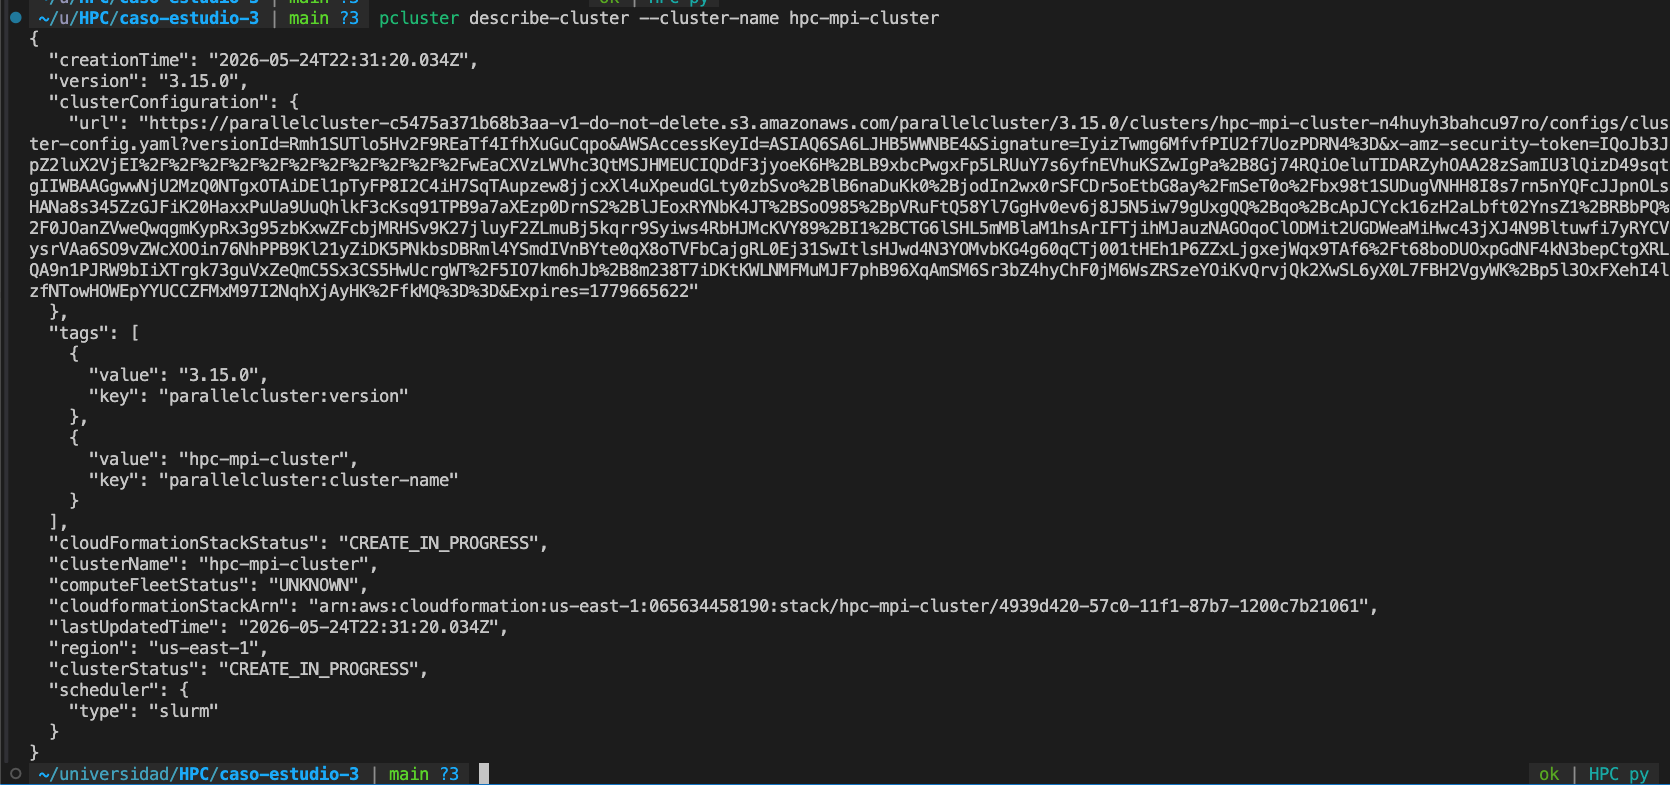
\includegraphics[width=\textwidth]{images/deploying_parallelcluster.png}
\caption{Despliegue del clúster con \texttt{pcluster create-cluster}.}
\label{fig:deploy}
\end{figure}

\subsection{Conexión al HeadNode}

Una vez en estado \texttt{CREATE\_COMPLETE}, se obtuvo la IP pública del HeadNode con:

\begin{verbatim}
pcluster describe-cluster --cluster-name hpc-mpi-cluster \
  --query 'headNode.publicIpAddress' --output text
# "3.235.161.247"
\end{verbatim}

y la conexión se realizó por SSH usando la clave generada previamente:

\begin{verbatim}
ssh -i ~/.ssh/hpc-mpi-key.pem ec2-user@3.235.161.247
\end{verbatim}

\begin{figure}[H]
\centering
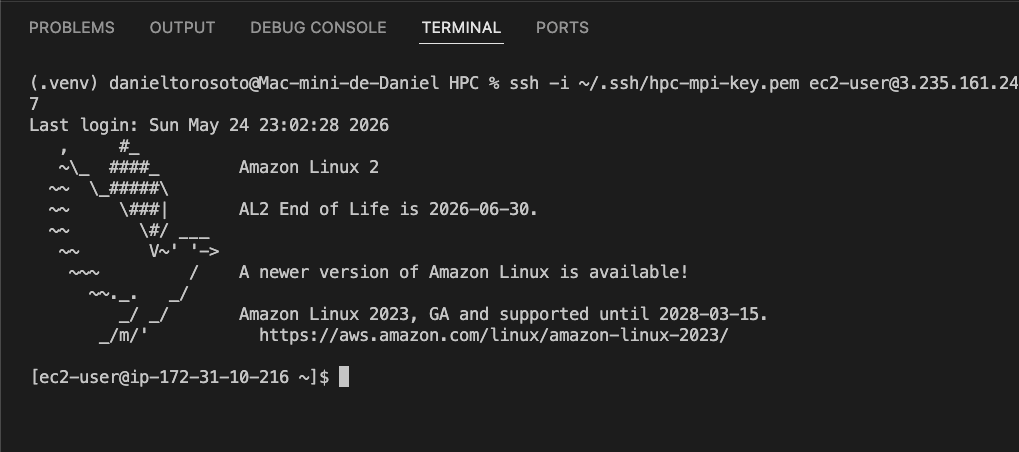
\includegraphics[width=\textwidth]{images/SSH_connection.png}
\caption{Conexión SSH al HeadNode tras consultar su IP pública.}
\label{fig:ssh}
\end{figure}

\subsection{Transferencia del código al EFS compartido}

El proyecto completo (código fuente, Makefile y scripts) se copió al directorio EFS compartido \texttt{/shared} mediante \texttt{scp}. Una vez allí, los nodos de cómputo lo ven automáticamente sin necesidad de copias adicionales:

\begin{verbatim}
scp -i ~/.ssh/hpc-mpi-key.pem -r \
  /Users/danieltorosoto/universidad/HPC/caso-estudio-3 \
  ec2-user@3.235.161.247:/shared/caso-estudio-3
\end{verbatim}

\begin{figure}[H]
\centering
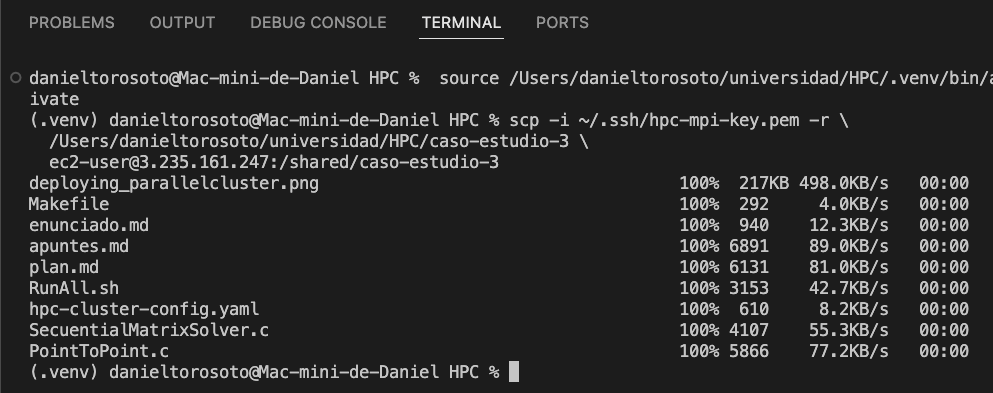
\includegraphics[width=\textwidth]{images/SCP_to_headnode.png}
\caption{Transferencia del proyecto al directorio compartido \texttt{/shared} del HeadNode.}
\label{fig:scp}
\end{figure}

\subsection{Asignación de recursos con Slurm}

Tras compilar el proyecto con \texttt{make}, se solicitó una asignación interactiva de recursos a Slurm. El comando ejecutado en la práctica fue:

\begin{verbatim}
salloc --nodes=3 --ntasks=6 --ntasks-per-node=2 --partition=compute
\end{verbatim}

Esto reserva los 3 nodos de cómputo simultáneamente, con 2 tareas por nodo, para un total de 6 procesos MPI disponibles (límite natural impuesto por la configuración: 3 nodos $\times$ 2 vCPUs/nodo $= 6$ vCPUs). Con esta asignación abierta, todas las llamadas subsiguientes a \texttt{mpirun} se distribuyen sobre los nodos reservados.

\begin{figure}[H]
\centering
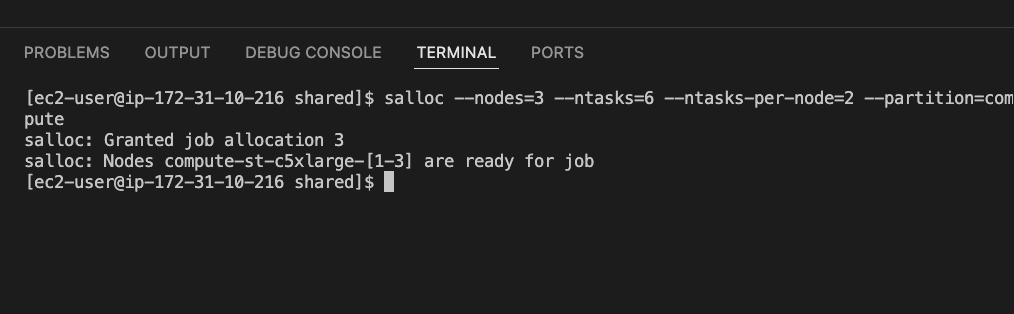
\includegraphics[width=\textwidth]{images/salloc_for_3_nodes.png}
\caption{Asignación de recursos con \texttt{salloc} para 3 nodos y 6 tareas.}
\label{fig:salloc}
\end{figure}

\subsection{Ejecución del benchmark}

Por último, el barrido completo de pruebas se lanzó en segundo plano con \texttt{nohup}, lo que permite que la sesión SSH pueda cerrarse sin abortar el proceso:

\begin{verbatim}
nohup bash RunAll.sh > runall.log 2>&1 &
\end{verbatim}

\begin{figure}[H]
\centering
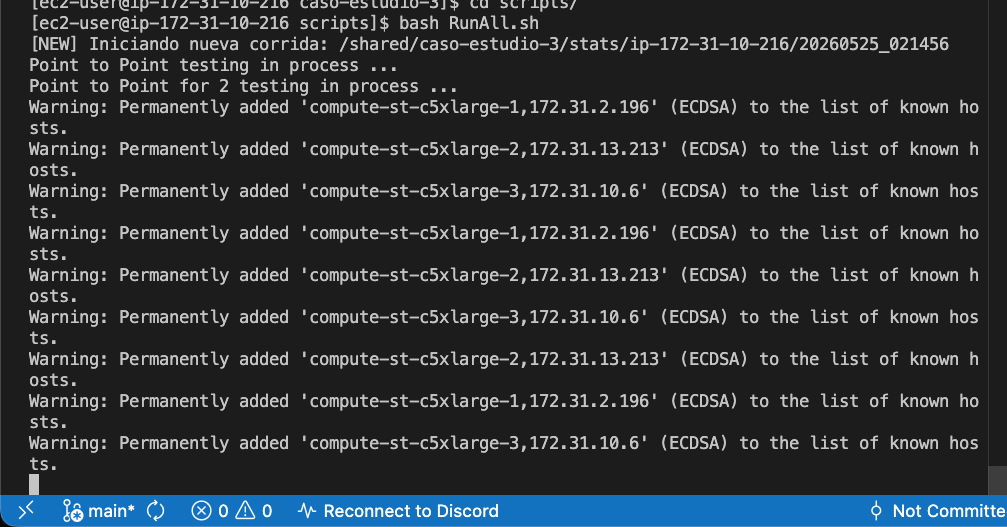
\includegraphics[width=\textwidth]{images/cluster_running_benchmark.png}
\caption{Ejecución del benchmark en background sobre el clúster.}
\label{fig:running}
\end{figure}

Al concluir la corrida, los CSV resultantes se recuperaron a la máquina local con:

\begin{verbatim}
scp -i ~/.ssh/hpc-mpi-key.pem -r \
  ec2-user@3.235.161.247:/shared/caso-estudio-3/stats \
  /Users/danieltorosoto/universidad/HPC/caso-estudio-3/stats/
\end{verbatim}

% ─────────────────────────────────────────────────────────────────────────────
\section{Pruebas}

A continuación se presentan los tiempos de ejecución (en segundos) medidos sobre el clúster, con 7 repeticiones por configuración. Los tamaños evaluados son: \textbf{504, 1008, 1296, 1608, 2004, 2304, 2604, 3000, 3300, 3600 y 4008}. La fila \textbf{Pr} corresponde al promedio sobre las 7 corridas y la fila \textbf{Speedup} es la razón $T_{seq}(n) / T_p(n)$ respecto al promedio secuencial de la Tabla~\ref{tab:secuencial}.

\subsection{Secuencial monolítico}

\begin{table}[H]
\centering
\tiny
\begin{tabular}{|c|c|c|c|c|c|c|c|c|c|c|c|}
\hline
\multicolumn{12}{|c|}{\textbf{Secuencial monolítico (1 nodo)}} \\
\hline
\textbf{Dimensión} & \textbf{504} & \textbf{1008} & \textbf{1296} & \textbf{1608} & \textbf{2004} & \textbf{2304} & \textbf{2604} & \textbf{3000} & \textbf{3300} & \textbf{3600} & \textbf{4008} \\
\hline
1 & 0.8106 & 12.3060 & 27.0610 & 57.3761 & 95.3988 & 176.7559 & 195.9331 & 389.4349 & 432.1465 & 678.6314 & 945.0613 \\
2 & 0.8021 & 12.0140 & 26.4754 & 57.2960 & 96.5203 & 176.9417 & 195.6262 & 389.2148 & 433.9327 & 678.9654 & 944.9075 \\
3 & 0.8008 & 11.7629 & 26.8397 & 57.7502 & 95.8755 & 176.4996 & 195.7034 & 392.1800 & 430.9143 & 678.8128 & 945.8382 \\
4 & 0.8125 & 11.7242 & 27.5700 & 56.6952 & 95.5283 & 176.0975 & 195.9362 & 390.2106 & 429.4717 & 677.3248 & 945.7674 \\
5 & 0.7977 & 11.7082 & 27.5933 & 57.0412 & 96.3679 & 175.7092 & 195.7642 & 389.1404 & 431.3241 & 679.0673 & 944.3342 \\
6 & 0.7971 & 12.0546 & 28.2674 & 56.3694 & 94.9194 & 175.9146 & 196.4258 & 389.5462 & 432.2447 & 677.3263 & 941.9913 \\
7 & 0.7995 & 12.9266 & 27.1167 & 56.6794 & 95.0250 & 176.7734 & 196.0549 & 390.7890 & 432.2724 & 679.6710 & 945.9243 \\
\hline
\textbf{Pr} & \textbf{0.8029} & \textbf{12.0710} & \textbf{27.2748} & \textbf{57.0297} & \textbf{95.6622} & \textbf{176.3845} & \textbf{195.9205} & \textbf{390.0737} & \textbf{431.7581} & \textbf{678.5427} & \textbf{944.8320} \\
\hline
\end{tabular}
\caption{Tiempos del binario secuencial monolítico ejecutado en un único nodo del clúster.}
\label{tab:secuencial}
\end{table}

\subsection{MPI Point-to-Point --- 2 procesos}

\begin{table}[H]
\centering
\tiny
\begin{tabular}{|c|c|c|c|c|c|c|c|c|c|c|c|}
\hline
\multicolumn{12}{|c|}{\textbf{MPI Point-to-Point --- 2 procesos}} \\
\hline
\textbf{Dim} & \textbf{504} & \textbf{1008} & \textbf{1296} & \textbf{1608} & \textbf{2004} & \textbf{2304} & \textbf{2604} & \textbf{3000} & \textbf{3300} & \textbf{3600} & \textbf{4008} \\
\hline
1 & 0.0740 & 1.1404 & 6.8542 & 18.3174 & 34.1801 & 70.2925 & 80.0321 & 130.5400 & 169.4479 & 243.8874 & 325.6519 \\
2 & 0.0786 & 1.1559 & 8.4621 & 18.2545 & 36.3381 & 70.4790 & 82.0369 & 133.4042 & 172.0957 & 244.6817 & 326.1514 \\
3 & 0.0755 & 1.1292 & 6.9728 & 18.5749 & 36.1755 & 67.3961 & 81.9096 & 131.5066 & 169.4137 & 242.1031 & 325.6040 \\
4 & 0.0745 & 1.1796 & 8.0887 & 17.4019 & 36.1874 & 68.4356 & 81.5723 & 131.4370 & 169.9215 & 242.1586 & 319.4499 \\
5 & 0.0747 & 1.1743 & 8.3806 & 18.8673 & 35.1995 & 69.6396 & 80.4419 & 123.5418 & 169.6436 & 242.8427 & 322.6000 \\
6 & 0.0782 & 1.1888 & 8.4785 & 18.4682 & 35.1357 & 67.6840 & 80.3217 & 129.4407 & 171.8913 & 244.0642 & 322.6987 \\
7 & 0.0770 & 1.2002 & 8.2369 & 18.5228 & 35.1443 & 70.5051 & 81.1060 & 132.2446 & 171.6062 & 244.4162 & 326.4506 \\
\hline
\textbf{Pr} & \textbf{0.0761} & \textbf{1.1669} & \textbf{7.9248} & \textbf{18.3438} & \textbf{35.4801} & \textbf{69.2046} & \textbf{81.0601} & \textbf{130.3021} & \textbf{170.5743} & \textbf{243.4506} & \textbf{324.0866} \\
\hline
\textbf{Speedup} & \textbf{10.55} & \textbf{10.34} & \textbf{3.44} & \textbf{3.11} & \textbf{2.70} & \textbf{2.55} & \textbf{2.42} & \textbf{2.99} & \textbf{2.53} & \textbf{2.79} & \textbf{2.92} \\
\hline
\end{tabular}
\caption{Tiempos y speedup del binario MPI con 2 procesos distribuidos en el clúster.}
\label{tab:p2p2}
\end{table}

\subsection{MPI Point-to-Point --- 4 procesos}

\begin{table}[H]
\centering
\tiny
\begin{tabular}{|c|c|c|c|c|c|c|c|c|c|c|c|}
\hline
\multicolumn{12}{|c|}{\textbf{MPI Point-to-Point --- 4 procesos}} \\
\hline
\textbf{Dim} & \textbf{504} & \textbf{1008} & \textbf{1296} & \textbf{1608} & \textbf{2004} & \textbf{2304} & \textbf{2604} & \textbf{3000} & \textbf{3300} & \textbf{3600} & \textbf{4008} \\
\hline
1 & 0.0554 & 0.5946 & 3.9423 & 8.8963 & 18.2499 & 35.1650 & 40.1974 & 66.8508 & 86.5083 & 120.7626 & 161.7219 \\
2 & 0.0650 & 0.5970 & 3.8523 & 9.0573 & 18.1084 & 35.0290 & 39.8755 & 65.4085 & 86.3313 & 121.4657 & 163.3144 \\
3 & 0.0647 & 0.5910 & 4.1355 & 9.1250 & 17.8460 & 35.2893 & 40.1333 & 66.4733 & 85.6070 & 123.0662 & 162.8193 \\
4 & 0.0654 & 0.5912 & 2.2866 & 8.8631 & 18.1324 & 35.4011 & 41.0048 & 65.0372 & 86.5912 & 122.1995 & 163.9298 \\
5 & 0.0661 & 0.5859 & 4.3168 & 9.3068 & 18.2486 & 35.9183 & 40.0194 & 65.4405 & 85.5784 & 121.8314 & 161.8108 \\
6 & 0.0646 & 0.5761 & 3.9591 & 8.5487 & 17.5297 & 34.1021 & 40.6271 & 66.1973 & 85.1920 & 121.5897 & 161.7428 \\
7 & 0.0557 & 0.5813 & 3.9727 & 8.8045 & 17.9466 & 34.5421 & 40.3667 & 66.0786 & 86.6480 & 121.6881 & 162.1290 \\
\hline
\textbf{Pr} & \textbf{0.0624} & \textbf{0.5882} & \textbf{3.7807} & \textbf{8.9431} & \textbf{18.0088} & \textbf{35.0638} & \textbf{40.3177} & \textbf{65.9266} & \textbf{86.0652} & \textbf{121.8005} & \textbf{162.4954} \\
\hline
\textbf{Speedup} & \textbf{12.86} & \textbf{20.52} & \textbf{7.21} & \textbf{6.38} & \textbf{5.31} & \textbf{5.03} & \textbf{4.86} & \textbf{5.92} & \textbf{5.02} & \textbf{5.57} & \textbf{5.81} \\
\hline
\end{tabular}
\caption{Tiempos y speedup del binario MPI con 4 procesos distribuidos en el clúster.}
\label{tab:p2p4}
\end{table}

\subsection{MPI Point-to-Point --- 6 procesos}

\begin{table}[H]
\centering
\tiny
\begin{tabular}{|c|c|c|c|c|c|c|c|c|c|c|c|}
\hline
\multicolumn{12}{|c|}{\textbf{MPI Point-to-Point --- 6 procesos}} \\
\hline
\textbf{Dim} & \textbf{504} & \textbf{1008} & \textbf{1296} & \textbf{1608} & \textbf{2004} & \textbf{2304} & \textbf{2604} & \textbf{3000} & \textbf{3300} & \textbf{3600} & \textbf{4008} \\
\hline
1 & 0.0771 & 0.4203 & 2.6642 & 5.9893 & 11.9676 & 23.7609 & 27.5135 & 43.3428 & 57.8124 & 80.4054 & 107.8654 \\
2 & 0.0763 & 0.4353 & 2.7624 & 5.9362 & 11.8902 & 23.3436 & 26.7608 & 43.5978 & 57.4197 & 80.6308 & 108.3422 \\
3 & 0.0661 & 0.4095 & 2.6407 & 6.0960 & 11.9231 & 23.3406 & 26.7818 & 43.6466 & 56.6631 & 81.6137 & 108.3984 \\
4 & 0.0677 & 0.4031 & 2.6151 & 6.1003 & 11.6947 & 23.6634 & 26.7407 & 43.9491 & 57.6445 & 81.0214 & 108.4100 \\
5 & 0.0667 & 0.4203 & 2.4444 & 6.1089 & 11.9417 & 23.9487 & 26.9129 & 43.6005 & 58.1408 & 82.3627 & 108.8173 \\
6 & 0.0768 & 0.4196 & 2.8927 & 5.8542 & 11.9727 & 23.5043 & 27.0200 & 43.5848 & 57.6752 & 81.2825 & 108.1142 \\
7 & 0.0662 & 0.4128 & 2.7499 & 5.9382 & 12.2013 & 23.3337 & 27.1920 & 43.5284 & 57.3770 & 81.4664 & 107.5994 \\
\hline
\textbf{Pr} & \textbf{0.0710} & \textbf{0.4173} & \textbf{2.6813} & \textbf{6.0033} & \textbf{11.9416} & \textbf{23.5564} & \textbf{26.9888} & \textbf{43.6071} & \textbf{57.5333} & \textbf{81.2547} & \textbf{108.2210} \\
\hline
\textbf{Speedup} & \textbf{11.31} & \textbf{28.93} & \textbf{10.17} & \textbf{9.50} & \textbf{8.01} & \textbf{7.49} & \textbf{7.26} & \textbf{8.95} & \textbf{7.50} & \textbf{8.35} & \textbf{8.73} \\
\hline
\end{tabular}
\caption{Tiempos y speedup del binario MPI con 6 procesos distribuidos en el clúster (2 procesos por nodo).}
\label{tab:p2p6}
\end{table}

% ─────────────────────────────────────────────────────────────────────────────
\section{Gráficas comparativas}

\subsection{Tiempo de ejecución}

\begin{figure}[H]
\centering

\includegraphics[width=\textwidth]{charts/tiempo_ejecucion.png}
\caption{Tiempo de ejecución en función de la dimensión de la matriz para el binario secuencial y las tres configuraciones MPI.}
\label{fig:tiempo}
\end{figure}

La gráfica de tiempo muestra cómo crece el costo del producto matricial al aumentar $N$. La curva secuencial domina ampliamente a las paralelas y diverge rápidamente: para $N = 4008$ el secuencial supera los 940 segundos, mientras que la versión con 6 procesos se mantiene por debajo de los 110 segundos. Las tres curvas paralelas presentan la misma forma cúbica del secuencial, pero con una pendiente mucho menor que depende del número de procesos.

\subsection{Speedup}

\begin{figure}[H]
\centering
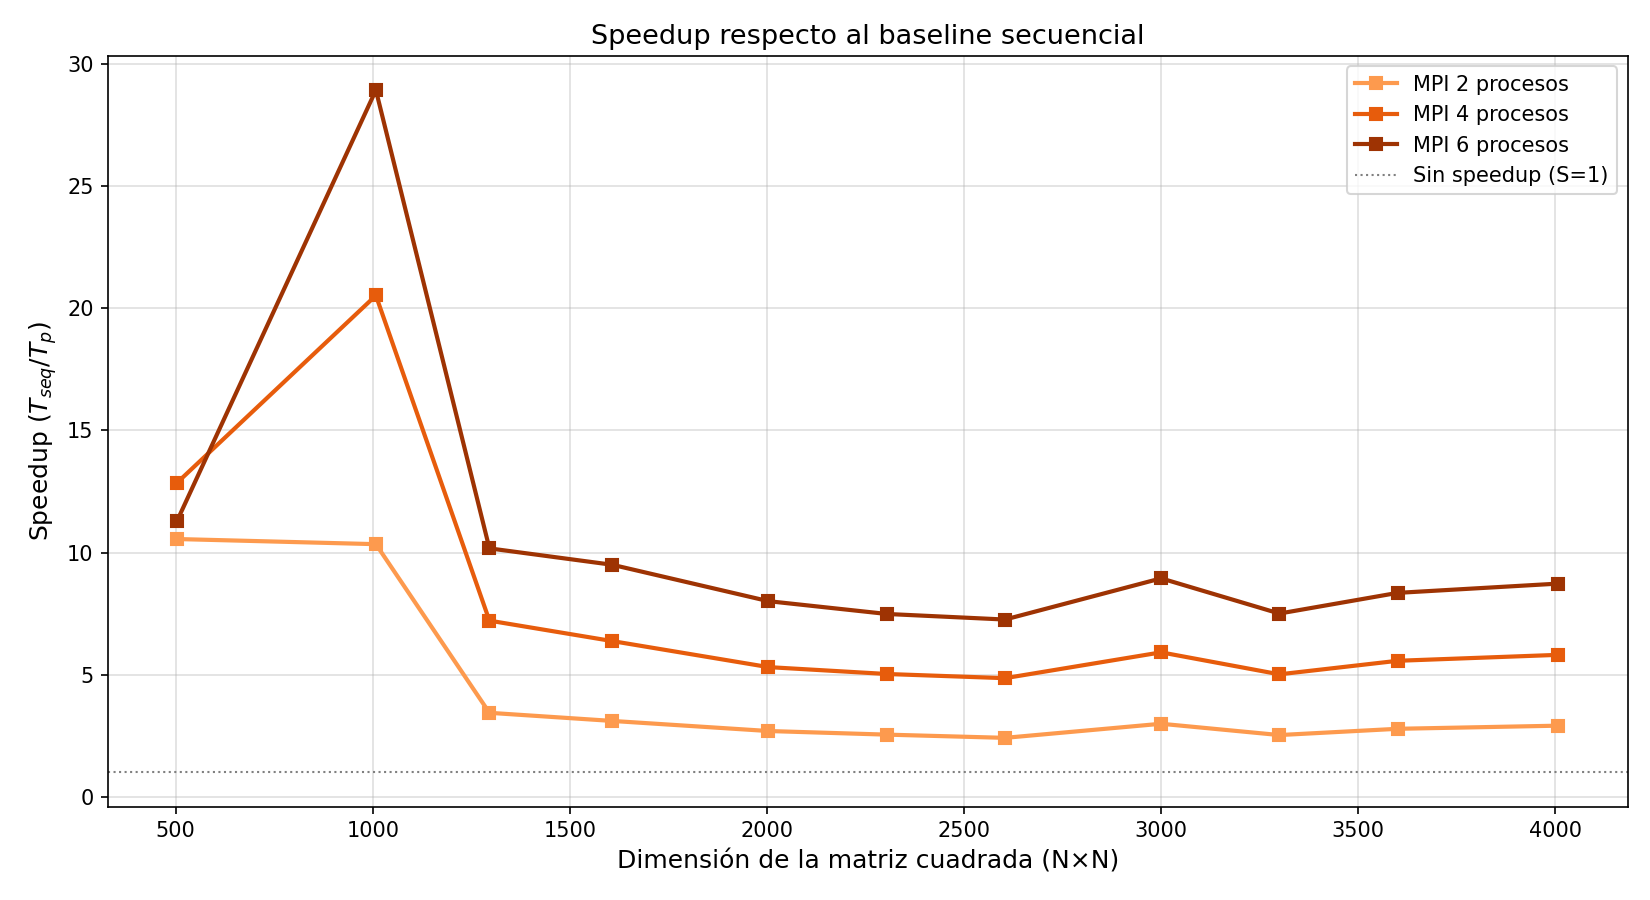
\includegraphics[width=\textwidth]{charts/speedup.png}
\caption{Speedup respecto al baseline secuencial monolítico, en función de la dimensión de la matriz, para 2, 4 y 6 procesos MPI.}
\label{fig:speedup}
\end{figure}

La gráfica de speedup es la herramienta más directa para evaluar la ganancia obtenida con MPI. Dos observaciones destacan:

\begin{enumerate}
    \item Para las matrices más pequeñas (504 y 1008) las tres curvas presentan un pico marcado, llegando a valores entre $10\times$ y $29\times$. Estos valores no son representativos de una ganancia ``pura'' de paralelización, sino del costo de inicialización del binario secuencial (alocación y llenado de matrices) frente al MPI, donde el grueso del tiempo es comunicación. Se incluyen para no descartar datos, pero el análisis se concentra en las dimensiones grandes.
    \item A partir de $N \geq 1296$ las tres curvas se estabilizan claramente: 2 procesos rondan un speedup de $2.5$--$3.4\times$, 4 procesos entre $4.9$ y $7.2\times$, y 6 procesos entre $7.3$ y $10.2\times$. La separación entre las tres curvas es consistente y refleja la ganancia real del paralelismo.
\end{enumerate}

\subsection{Heatmap de speedup}

\begin{figure}[H]
\centering
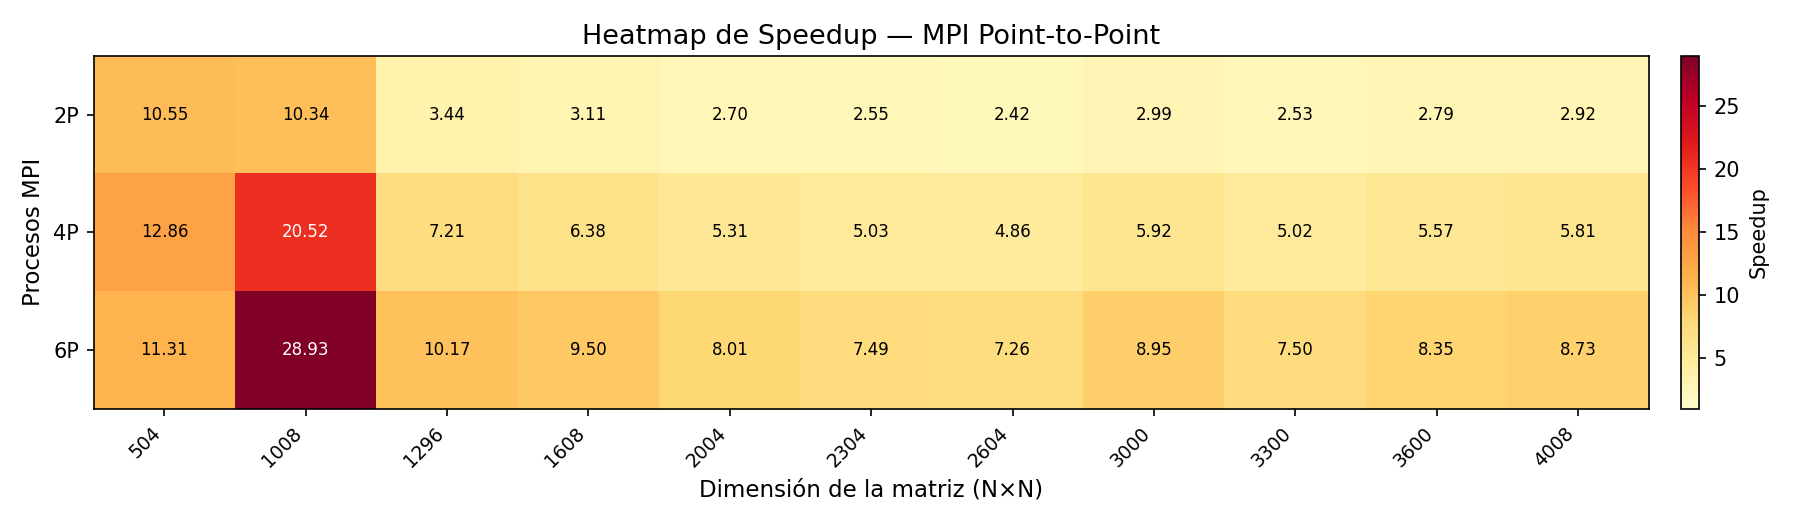
\includegraphics[width=\textwidth]{charts/heatmap_speedup.png}
\caption{Heatmap de speedup: cada celda muestra $S_p$ para una combinación de configuración (filas) y dimensión de matriz (columnas).}
\label{fig:heatmap}
\end{figure}

El heatmap resume en una sola vista toda la matriz de resultados. Las zonas más oscuras corresponden a las celdas con speedup más alto y se concentran principalmente en la combinación de 6 procesos $+$ matrices entre 1296 y 4008. La ``zona estable'' (a partir de $N \geq 1296$) muestra un patrón ordenado donde el speedup crece monótonamente con el número de procesos, lo que es coherente con la teoría: a mayor cómputo total, mejor amortización del overhead de comunicación.
% ─────────────────────────────────────────────────────────────────────────────
\section{Análisis de Resultados}

\subsection{Comportamiento del speedup observado}

Para matrices grandes ($N \geq 2000$), los speedups observados son consistentes y crecen con el número de procesos. Tomando $N = 4008$ como referencia, los valores son: $S_2 = 2.92$, $S_4 = 5.81$ y $S_6 = 8.73$. Las relaciones entre configuraciones MPI son particularmente informativas: pasar de 2 a 4 procesos aporta un factor de $5.81/2.92 \approx 1.99\times$, casi exactamente el factor 2 esperado al duplicar recursos. De 4 a 6 procesos se obtiene un factor $8.73/5.81 \approx 1.50\times$, también muy cercano a la relación ideal $6/4 = 1.50$. Esto sugiere que el algoritmo está aprovechando casi por completo los recursos adicionales del clúster.

\subsection{Picos en matrices pequeñas}

Para $N \in \{504, 1008\}$ el speedup absoluto supera el número de procesos disponibles (hasta $29\times$ con 6 procesos sobre $N=1008$). Este fenómeno, conocido como \emph{speedup superlineal}, suele explicarse por dos factores: (i) los costos fijos de inicialización del binario secuencial (asignación, llenado de matrices con \texttt{rand()} y liberación de memoria) representan una fracción comparativamente alta del tiempo para matrices pequeñas; y (ii) cuando el problema se reparte entre procesos, cada porción puede caber en niveles más rápidos de la jerarquía de memoria de cada nodo, mejorando la utilización de caché por proceso. Para los tamaños grandes el cómputo domina y la curva ``aterriza'' en valores razonables.

\subsection{Impacto del overhead de comunicación}

En MPI, antes de comenzar a calcular, el rank 0 debe enviar a cada worker su batch de filas de $A$ \emph{más} la matriz $B$ completa (tag 1). Este último envío es proporcional a $n^2$ enteros por cada worker, lo que para $N = 4008$ representa cerca de 64\,MB transferidos por la red por cada worker. A pesar de este costo, los nodos están en la misma subred (latencia intra-AZ) y el ancho de banda intra-AWS basta para que el envío se amortice contra los $\mathcal{O}(n^3)$ operaciones de cómputo asignadas a cada worker. En matrices muy pequeñas esta amortización falla: el tiempo de comunicación es comparable al tiempo de cómputo y el escalado se desvía del ideal.

\subsection{Configuración de Slurm y techo de paralelismo}

La asignación \texttt{salloc --nodes=3 --ntasks=6 --ntasks-per-node=2} fija el techo en 6 procesos MPI, exactamente igual al número total de vCPUs del clúster (3 nodos $\times$ 2 vCPUs/nodo). Intentar lanzar más procesos sin overcommit requeriría: (i) aumentar el número de nodos (\texttt{MaxCount}), o (ii) cambiar el tipo de instancia a uno con más vCPUs por nodo (por ejemplo \texttt{c5.xlarge} con 4 vCPUs). El comportamiento casi lineal observado hasta $p = 6$ sugiere que ampliar la cota probablemente seguiría aportando speedup adicional para problemas suficientemente grandes.

\subsection{Comparación cualitativa con paralelismo de memoria compartida}

En el Caso de Estudio 1 se evaluaron implementaciones de memoria compartida (hilos POSIX y \texttt{fork} con \texttt{mmap}) sobre un Apple M4 de 10 núcleos. Aquellas variantes no tienen costo explícito de transferencia de datos porque los workers leen las matrices directamente de memoria compartida, y por eso alcanzaban speedups cercanos al ideal con menor overhead. La implementación MPI, en cambio, paga el costo de comunicación por la red, pero a cambio puede agregar memoria y cómputo de varias máquinas independientes, lo que permite escalar problemas que no caben en una sola. Para este caso (matriz $4008 \times 4008$, $\approx 64$\,MB por matriz) el clúster cumple la promesa: la versión MPI con 6 procesos no es más rápida que un Apple M4 con 8--16 hilos, pero demuestra que la arquitectura distribuida es viable y que el costo de comunicación es manejable cuando la relación cómputo/comunicación es favorable.

% ─────────────────────────────────────────────────────────────────────────────
\section{Conclusiones}

\begin{enumerate}
    \item \textbf{Escalabilidad casi lineal entre configuraciones MPI}. Para matrices $N \geq 2000$, duplicar el número de procesos (de 2 a 4) duplica el speedup, y pasar a 6 procesos lo aumenta en un factor cercano a $1.5\times$, ambos coherentes con la relación ideal entre recursos. El algoritmo punto a punto implementado aprovecha los nodos del clúster de manera efectiva dentro del rango de procesos disponible.

    \item \textbf{El overhead de comunicación domina en matrices pequeñas}. Para $N \leq 1296$ los tiempos de envío de $A$ y $B$ por la red son comparables al tiempo de cómputo, y el speedup observado no es representativo del paralelismo real. La paralelización distribuida sólo compensa para problemas suficientemente grandes.

    \item \textbf{Configuración óptima dentro del clúster: 6 procesos en 3 nodos}. Con la configuración \texttt{c7i-flex.large} y \texttt{ntasks-per-node=2}, el techo natural es 6 procesos. En esa configuración se alcanza $S_6 = 8.73$ para $N = 4008$ respecto al baseline secuencial monolítico. Para escalar más allá habría que cambiar el tipo de instancia o aumentar el número de nodos.

    \item \textbf{AWS ParallelCluster reduce la complejidad operacional pero introduce ataduras}. El despliegue requirió Python 3.9 específicamente, par de claves SSH, configuración YAML, manejo de subredes y revisión del estado del stack en CloudFormation. A cambio, una vez en funcionamiento, Slurm y EFS permiten ejecutar el benchmark exactamente como se haría en un clúster on-premise, sin necesidad de scripts manuales de distribución de binarios.

    \item \textbf{EFS resuelve la distribución del binario, pero no la del dato}. El sistema de archivos compartido elimina la fricción del despliegue (basta con \texttt{make} en el HeadNode), pero la matriz $B$ debe seguir siendo enviada explícitamente a cada worker en cada corrida. Una optimización futura sería leer $B$ directamente del EFS desde cada worker, evitando la transferencia por MPI.

    \item \textbf{\texttt{MPI\_Wtime} resuelve la advertencia del enunciado sobre relojes heterogéneos}. Toda la medición ocurre desde el rank 0, sobre un único reloj, evitando comparar tiempos entre nodos con tasas de avance diferentes.
\end{enumerate}

% ─────────────────────────────────────────────────────────────────────────────
\newpage
\section{Bibliografía}

\begin{thebibliography}{9}

    \bibitem{cortez}
    Cortéz, A. (2004). Teoría de la complejidad computacional y teoría de la información.
    \textit{Revista de Investigación de Sistemas e Informática}, 1(1), 102--105.
    \url{https://revistasinvestigacion.unmsm.edu.pe/index.php/sistem/article/view/3216}

    \bibitem{ferestrepoca}
    Ferestrepoca. (2019). Paradigmas de programación paralela.
    \url{http://ferestrepoca.github.io/paradigmas-de-programacion/paralela/paralela_teoria/index.html}

    \bibitem{lopez}
    López, A. (2017). Introducción al High Performance Computing. \textit{Encamina Blog}.
    \url{https://blogs.encamina.com/por-una-nube-sostenible/introduccion-al-high-performance-computing/}

    \bibitem{amdahl}
    Amdahl, G. M. (1967). Validity of the single processor approach to achieving large scale computing capabilities.
    \textit{Proceedings of AFIPS Spring Joint Computer Conference}, pp. 483--485.

    \bibitem{mpiforum}
    MPI Forum. (2023). \textit{MPI: A Message-Passing Interface Standard}, Version 5.0.
    \url{https://www.mpi-forum.org/}

    \bibitem{openmpi}
    The Open MPI Project. (2024). \textit{Open MPI: Open Source High Performance Computing}.
    \url{https://www.open-mpi.org/}

    \bibitem{mpitutorial}
    Kendall, W. (2014). \textit{MPI Tutorial}.
    \url{https://github.com/mpitutorial/mpitutorial}

    \bibitem{parallelcluster}
    Amazon Web Services. (2024). \textit{AWS ParallelCluster User Guide}.
    \url{https://docs.aws.amazon.com/parallelcluster/}

\end{thebibliography}

\end{document}
